\documentclass{article}
\usepackage[top=0pt,left=0pt,bottom=0pt,right=0pt,paperwidth=10cm,paperheight=7cm]{geometry}
\usepackage{tikz}
\usetikzlibrary{decorations.pathmorphing}
\pagestyle{empty}
\begin{document}
\centering%
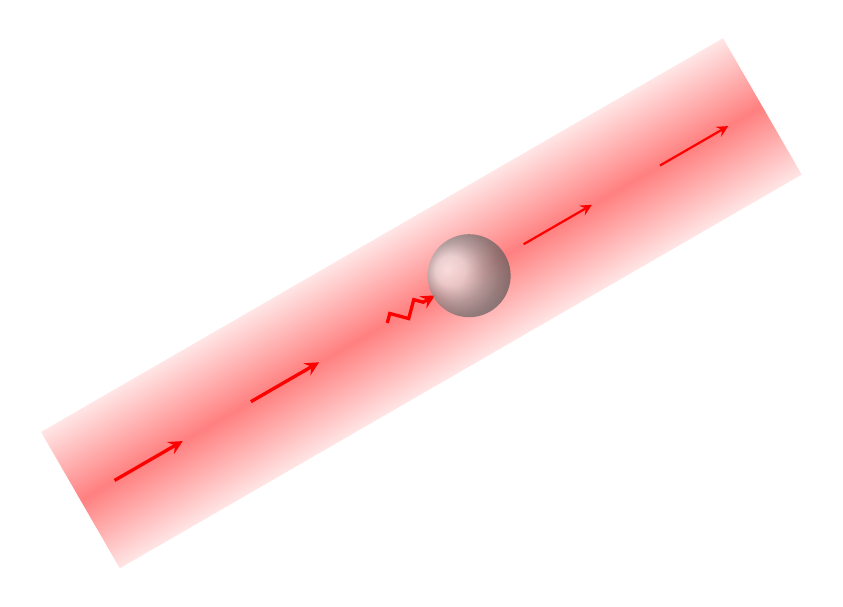
\begin{tikzpicture}
\path[use as bounding box] (-5,-3.5) rectangle ++(10,7);
\begin{scope}[transform canvas={rotate=30}]
\shade[top color=red!10,bottom color=red!10,middle color=red!50] (-5,-1) rectangle ++(10,2);
\foreach \x in {-4.5,-2.5}{
  \draw[very thick,red,-stealth] (\x,0) -- ++(1,0);
}
\foreach \x in {1.5,3.5}{
  \draw[thick,red,-stealth] (\x,0) -- ++(1,0);
}

\draw[very thick,red,-stealth,decoration=zigzag,decorate] (-0.5,0) -- ++(0.7,0);
\shade[ball color=gray!30,opacity=0.7] (0.7,0) circle(15pt);
\end{scope}
\end{tikzpicture}
\end{document}
